\documentclass[a4paper,12pt]{article}
\usepackage{t1enc}
\usepackage[longnamesfirst, round]{natbib}  % Bindet den natbib-standard fuer das Zitieren ein
\usepackage{epsfig}
\usepackage[utf8]{inputenc}   % Ermoeglicht Sonderzeichen direkt einzugeben
\usepackage[T1]{fontenc}        % Garantiert saubere Worttrennung bei Umlauten etc.
\usepackage{color}              % Farbpaket
\usepackage{amsmath,amsfonts,amssymb}   % ermoeglicht mathematische Sonderzeichen
\usepackage{ngerman}           % neue deutsche Rechtschreibung
\usepackage[english]{babel}     %
\usepackage{ae}                 %
\usepackage{graphicx}           % Ermoeglicht das Einbinden von Bildern in allen Formaten
\usepackage{longtable}          % zum erstellen von Tabellen ber mehrere Seiten
\usepackage{multirow}           % zum Verbinden von Zeilen innerhalb einer Tabelle
%\usepackage{pictexwd}           % PicTex, ein Graphikpaket
%\usepackage{pst-all, multido}   % psTricks, ein Graphikpaket
\usepackage{url}
\usepackage{float}
\usepackage{subcaption}
\usepackage{booktabs, caption}
\usepackage[flushleft]{threeparttable}

% ________________ EINRICHTEN DES DOKUMENTS ______________________%

\bibliographystyle{apalike}    % legt den Stil fuer das Inhaltsverzeichnis fest

\oddsidemargin 0.1in \evensidemargin 0.1in \textwidth 15.5cm \topmargin -0.4in \textheight 24.5cm
\parindent 0cm      % legt die Seitenraender fest

\pagestyle{plain}          % leere Kopfzeile, Seitennummer in der Mitte der Fusszeile

\newcommand{\bs}{\boldsymbol}  % shortcut zur Erzeugung von fetten Sympolen in der Mathe-Umgebung

\renewcommand{\baselinestretch}{1.25}
% 1,5 -facher Zeilenabstand (Standard ist 1,2-facher Zeilenabstand, also 1,2*1,25 = 1,5



\begin{document}

% ________________ TITELSEITE ______________________%


\pagenumbering{roman}   % roemische Zahlen zur Seitennumerierung

\begin{titlepage}       % Umgebung fuer Titelseite, frei gestaltbar

\thispagestyle{empty}   % keine Numerierung auf Titelseite


\begin{center}
\vspace*{2.5cm}
{\bf  \Large Effects of Unemployment Benefits and Uncertainty in Heterogeneous Models\\The Importance of Endogenous Duration of Unemployment} \\
\vspace*{3cm} 
Term paper for the \\ Project Module in Macroeconomics and Public Economics: Uncertainty and Volatility \\
of Prof. Dr. Benjamin Born and Junior-Prof. Dr. Markus Riegler  \\
\vspace*{0.5cm} 
Winter Term 2016/17\\
\end{center}

\vfill
\begin{flushright}
   \emph{Eric Lustenberger} \\
    \emph{Bonner Talweg 34}\\
    \emph{53113 Bonn}\\
   \emph{Stud Nr.: 2849851}\\
 \emph{M.Sc. Economics}\\

\end{flushright}



% 
% \begin{center}
% $ $			% oeffnet und schliesst eine Matheumgebung (Trick, um den Titel nach unten zu rutschen
% \vspace{4cm}
% 
% {\LARGE TITEL}
% \vskip 4cm
% 
% Diese Seite ist frei gestaltbar
% \end{center}

\end{titlepage}

\newpage                % erzwingt an dieser Stelle einen Seitenumbruch



% ________________ INHALTSVERZEICHNIS ______________________%


% \tableofcontents   %fuegt Automatisch ein Inhaltsverzeichnis ein
% 
% \newpage
% 


% ________________ HAUPTTEIL ______________________%


\pagenumbering{arabic}      % Seitenzahlen wieder arabisch numerieren
\setcounter{page}{1}        % Ruecksetzen des Seitenzahlzaehlers auf 1


\section{\"Uberschrift}
\label{Kapitel1}

\subsection{Unter\"Uberschrift}

\subsubsection*{UnterUnter\"Uberschrift}



Hier steht mal ein Text. Eine M\"oglichkeit des Zitierens ist, direkt
im Text die Quelle anzugeben \citep[see][pp.225-369]{key1}.
Andererseits schreiben \cite{key2}, dass man auch so zitieren kann.

In der Matheumgebung kann der oben (im Latex-Quellcode) genannte Shortcut verwendet
werden, um aus einem normalen $\beta$ ein fettes $\bs \beta$ zu
machen. Wichtige Gleichungen, die nochmal verwendet werden, sollten nummeriert werden, z.B.
\begin{equation}
\label{eq:ols}
   b = (x'x)x'y \;.
\end{equation}

Nebens\"achlicheres, auf das man sich nicht mehr bezieht, bleibt unnummeriert, also 
\begin{equation*}
   a = 1\;.
\end{equation*}
Nun kann man direkt auf die erste Gleichung als Gleichung~\eqref{eq:ols} verweisen mittels des zugewiesenen labels. In gleicher Weise kann man auf die Graphik~\ref{fig:ersteGraphik} bzw. Graphik~\ref{fig:andereGraphik} verweisen. Die Tilde zwischen \glqq Graphik\grqq{} und \glqq \verb|\ref{fig:andereGraphik}|\grqq{} verhindert, dass bei Zeilenumbr\"uchen die Zahl als erstes alleine in die neue Zeile rutscht. Ganz analog f\"ur die Tabelle~\ref{tab:Tabelle}. 



\section{Ben\"otigte Programme}

unter Windows:
\begin{itemize}
   \item Miktex (\url{http://miktex.org/})
   \item ein Editor, je nach Geschmack z.B. WinEdt (\url{http://www.winedt.com/}; kostenpflichtige Studentenversion) oder einen der vielen anderen verf\"ugbaren, z.B. TeXnicCenter (\url{www.texniccenter.org/})
   \item ghostview und ghostscript (\url{http://pages.cs.wisc.edu/~ghost/}
\end{itemize}
unter Linux:
\begin{itemize}
   \item Latex ist in den meisten Verteilungen enthalten, z.B. tetex in Suse (ggf. \"uber yast nachinstallieren)
   \item als Editor empfiehlt sich z.B. Kile
\end{itemize}
f\"ur die Literatur:\\
z.B. JabRef (\url{http://jabref.sourceforge.net/})


\section{Pr\"asentationen}

Beispiele f\"ur Pr\"asentationen mit dem Beamer-Style:

\url{http://www.informatik.uni-freiburg.de/~frank/latex-kurs/latex-kurs-3/Latex-Kurs-3.html}

\section{Model}

The setup is a basic \cite{aiyagari} model. 

\subsection{Consumer's Problem}

There is a continuum of ex-ante identical infinitely-lived consumers with population 1. Consumers maximize the discounted lifetime utility: 

\[ 
 max_{\{{ c_{i,t}, k_{i,t+1} }\}_{t = 0}^{\infty}} {\mathbb{E}} \sum_{i=0}^{\infty} \beta^{t}  u(c_{i,t}) 
 \]

where $\beta \in (0,1)$ is the discount factor, $ c_{t}$ is consumption at time t and $\mathbb{E[.]}$ is the expectation at time 0. 

Consumers are subject to uninsurable idiosyncratic risk. In each period they can be employed or unemployed. This process is governed by a transition matrix:
\[ \Pi = \begin{bmatrix}
1-\pi_{UE} & \pi_{UE} \\
 \pi_{EU} & 1-\pi_{EU}
\end{bmatrix}
\]

where $\pi_{UE}$ is the probability to find a job next period and $pi_{EU}$ is the layoff probability. 



Consumers are allowed to interact on the capital market and accumulate one type of asset: at . Furthermore, consumers can be employed, or unemployed at each point in time. They are therefore subject to the following budget constraint at each point in time: 
  \[ 
  c_{i,t} + k_{i,t+1} = (1 + r_{t} - \delta) k_{i,t} + w_{t} (1 - \tau_{t})  e_{i,t} + \mu w_{t} (1 - e_{i,t})
  \]
 where rt is the interest rate at time t, $\delta$ is the depreciation rate, $w_{t}$ is the wage at time t. 
Finally, consumers are constrained in their borrowing, $k_{min}$ denotes the minimum amount of capital consumers are required to hold at each point in time: 

   \[
   k_{i,t + 1} \geq \bar{k}
 	\]
	
\subsection{Firm's Problem}

The representative firm maximizes profits 
\[ \max_{\substack{K_{t},L_{t}}}F_{t}(K_{t},L_{t})-r_{t}K_{t}-w_{t}L_{t}
\]

Factor prices are obtained by taking the FOC's with respect to the aggregate capital stock and the aggregate labour, respectively: 
\[
r_{t} = \frac{\mathrm d F_{t}(K_{t},L_{t})}{\mathrm d K} = \alpha z (\tfrac{L_{t}}{K_{t}})^{1-\alpha} \]
\[
w_{t} = \frac{\mathrm d F_{t}(K_{t},L_{t})}{\mathrm d L} =(1-\alpha)z (\tfrac{K_{t}}{L_{t}})^{\alpha}
\]

\subsection{General Equilibrium}

The households take 

Euler equation:
\[ 
c_{i,t}^{- \sigma} \geq \beta (1+r -\delta){\mathbb{E}[c_{i,t+1}^{- \sigma}}]
\]
Budget constraint:
 \[ 
 c_{i,t} + k_{i,t+1} = (1 + r_{t} - \delta) k_{i,t} + w (1 - \tau)  e_{i,t} + \mu w (1 - e_{i,t})
 \]
Borrowing constraint:
  \[
  k_{i,t + 1} \geq k_{min}
	\]
Factor prices:
\[
r = \alpha z (\tfrac{L}{K})^{1-\alpha} \ \ \ w = (1-\alpha)z (\tfrac{K}{L})^{\alpha}
\]
Employment and Tax rate: 
\[
L = \tfrac{\pi_{UE}}{\pi_{UE}+\pi_{EU}} \ \ \ \ \  \tau = \mu \tfrac{1-L}{L}
\]
\section{Welfare analysis}
We want to compare the utility level of the same agent before and after the policy change. There are two challenges to overcome, firstly we need take transitions into account. It may be the case that during the transition phase from one steady state to the other, agents loose eventough in the end they are in a preferred steady state and therefore do not prefer the policy change taking the transition into account. Secondly, utility is a purely ordinal measure and therefore not quantifiable. 

For our presentation we have taken two different forms of measurement into account - Consumption equivalent and Cash equivalent. I will here only look at the Cash equivalent since it is a better measure.\footnote{The Consumption equivalent does weight different level's of consumption differently. A concave utility function implies that a consumption change of the same order is weighted differently by rich individuals with a high consumption to poor individuals with a low consumption.} 

  \begin{itemize}
\item {
  Transfer of $\Delta$ units of wealth in the first period
  }
  \end{itemize}
  
  \begin{equation}
  U^{2}(e,k) = U^{1}(e,k+\Delta) \nonumber
  \end{equation}
  
  \begin{itemize}
  \item {
  If $ \Delta>0 $ agents prefer the policy change $ (U^{2}) $, otherwise not.
  }
  \end{itemize}



\section{Results}

\subsection{Calibration}

I will use the KrusellandSmith calibration, which founded the basis of our analysis for the presentation. However, since I am not considering aggregate risk, I will use the job-finding probability of 0.4, which corresponds to an average unemployment duration of 2.5 quarters or 32.5 weeks. Note that this a rather high estimate of unemployment duration.\footnote{\cite{mukoyama} makes a calibration for the post 1980 US economy, has a job-finding probability of 0.26 corresponding to 17 weeks of unemployment, thus providing a better match for the real data.}
Other variables are, a discount factor $\beta = 0.99$, productivity $z = 1$, $\alpha = 0.36$, depreciation rate $\theta = 0.025$, the baseline employment $rate l=0.9$, the baseline replacement rate $\mu = 0.15$.


%_________________ ENDE DES HAUPTTEILS_________________%


\newpage


%_________________ Literaturverzeichnis _______________%

\addcontentsline{toc}{section}{References}        % Fuegt im Inhaltsverzeichnis "References" hinzu
\bibliography{bibexample}                         % Erstellt Literaturverzeichnis (bindet das file bibexample.bib ein

%_________________ Platz fuer Graphiken und Tabellen _______________%

\newpage

% Einfuegen einer Grafik
\begin{figure}
\caption{titel der Graphik} 
\label{fig:ersteGraphik}	%label, um spaeter auf die Graphiknummer zugreifen zu koennen
\centering
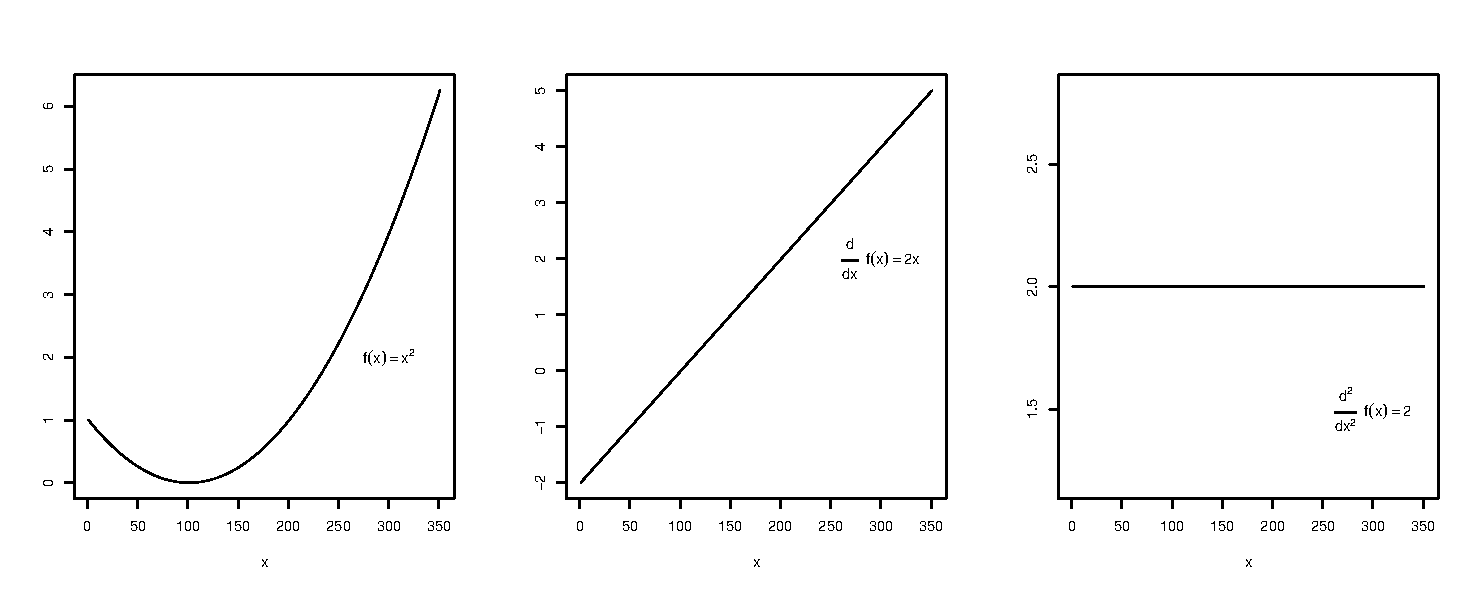
\includegraphics[width=6.5cm]{abb1.png}  % width legt Breite der Graphik fest

\begin{minipage}{0.8\linewidth}
\footnotesize{die Graphik sollte beschrieben werden, sodass man ohne den Text vorne zu lesen wei\ss{}, worum es geht: panel 1 zeigt die Funktion, panel 2 die erste Ableitung und Panel 3 die zweite Ableitung}
\end{minipage}

\end{figure}

\begin{figure}
\caption{titel der Graphik}
\label{fig:andereGraphik} \centering
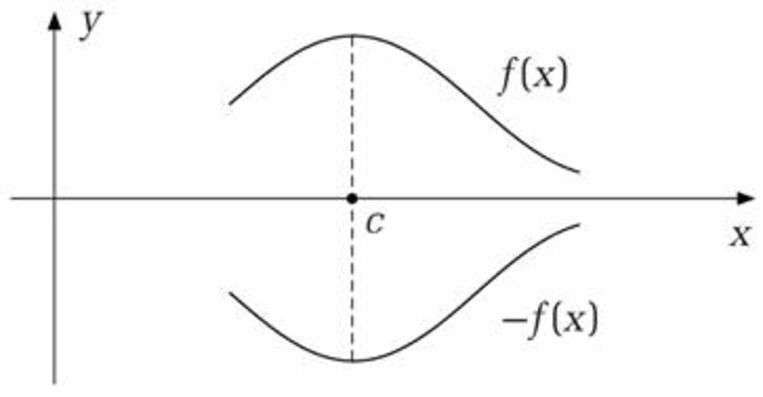
\includegraphics[angle=90,height=6.5cm]{abb2.jpg}  % angle dreht die Graphik, falls noetig; height legt die Hoehe der Graphik fest

\end{figure}

\begin{table}
\caption{Der Title der Tabelle}
\label{tab:Tabelle}
\centering
 \begin{tabular}{lc|r}
   Eine & kleine & Tabelle\\
\hline
   Text links & mittig & oder rechts \\
   & unterstrichen  & \\
\cline{2-2}
   \multicolumn{2}{c|}{\"uber zwei Spalten} & dritte Spalte \\
\end{tabular}   
\end{table}

   





\end{document}
